%% Created by Maple 17.01, Windows 7
%% Source Worksheet: applications,DCMotor
%% Generated: Thu Nov 21 14:49:36 CST 2013
\documentclass{article}
\usepackage{maplestd2e}
\def\emptyline{\vspace{12pt}}
\begin{document}
\pagestyle{empty}
\DefineParaStyle{Maple Heading 1}
\DefineParaStyle{Maple Text Output}
\DefineParaStyle{Maple Dash Item}
\DefineParaStyle{Maple Bullet Item}
\DefineParaStyle{Maple Normal}
\DefineParaStyle{Maple Heading 4}
\DefineParaStyle{Maple Heading 3}
\DefineParaStyle{Maple Heading 2}
\DefineParaStyle{Maple Warning}
\DefineParaStyle{Maple Title}
\DefineParaStyle{Maple Error}
\DefineCharStyle{Maple Hyperlink}
\DefineCharStyle{Maple 2D Math}
\DefineCharStyle{Maple Maple Input}
\DefineCharStyle{Maple 2D Output}
\DefineCharStyle{Maple 2D Input}
\begin{maplelatex}\begin{Maple Normal}{
\raisebox{0.9583333333333334in}{
\includegraphics[keepaspectratio,totalheight=11.11111111111111in,angle=-90]{DCMotorimage0.eps}}}\end{Maple Normal}
\end{maplelatex}
\begin{maplegroup}
\begin{center}
\begin{Maple Title}{
\textbf{DC Motor Control Design}}\end{Maple Title}
\end{center}
\end{maplegroup}
\begin{maplegroup}
\begin{Maple Normal}{
Given a model of a DC motor as a set of differential equations, we want to obtain both the transfer function and the state space model of the system. Then, we want to use the state space model to design a LQR controller and study the effect the R parameter in the LQR control design has on the controlled performance of the system.}\end{Maple Normal}

\end{maplegroup}
\begin{maplelatex}\begin{Maple Heading 2}{
\textbf{}System Definition\textbf{}}\end{Maple Heading 2}
\end{maplelatex}
\begin{maplelatex}\begin{Maple Bullet Item}{
\underline{}Parameters\underline{}}\end{Maple Bullet Item}
\end{maplelatex}
\begin{maplelatex}\begin{Maple Bullet Item}{
\underline{}Variables\underline{}}\end{Maple Bullet Item}
\end{maplelatex}
\begin{maplelatex}\begin{Maple Normal}{
System Models}\end{Maple Normal}
\end{maplelatex}
\begin{maplelatex}\begin{Maple Bullet Item}{
\underline{}Differential Equation Model\underline{}}\end{Maple Bullet Item}
\end{maplelatex}
\begin{maplelatex}\begin{Maple Bullet Item}{
\underline{}Transfer Function Model\underline{}\underline{}}\end{Maple Bullet Item}
\end{maplelatex}
\begin{maplelatex}\begin{Maple Bullet Item}{
\underline{}State Space Model\underline{}}\end{Maple Bullet Item}
\end{maplelatex}
\begin{maplelatex}\begin{Maple Bullet Item}{
\underline{}Model Analysis\underline{}}\end{Maple Bullet Item}
\end{maplelatex}
\begin{maplelatex}\begin{Maple Heading 2}{
LQR Control Design}\end{Maple Heading 2}
\end{maplelatex}
\begin{maplelatex}\begin{Maple Bullet Item}{
\underline{}Step Responses\underline{}}\end{Maple Bullet Item}
\end{maplelatex}
\begin{maplelatex}\begin{Maple Bullet Item}{
\underline{}How varying R affects the System Response\underline{}}\end{Maple Bullet Item}
\end{maplelatex}
\begin{maplelatex}\begin{Maple Heading 3}{
\textbf{}}\end{Maple Heading 3}
\end{maplelatex}
\begin{maplegroup}
\begin{center}
\begin{Maple Normal}{
\raisebox{6.722222222222222in}{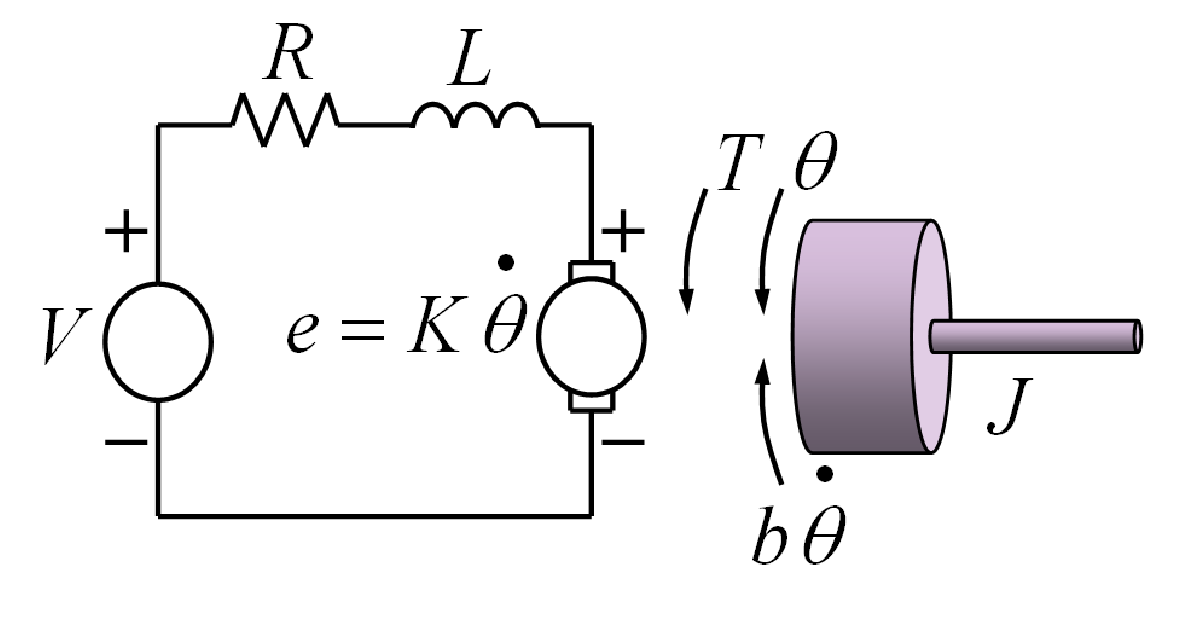
\includegraphics[keepaspectratio,totalheight=13.291666666666666in,angle=-90]{DCMotorimage1.eps}}}\end{Maple Normal}
\end{center}
\end{maplegroup}
\begin{maplelatex}\begin{Maple Normal}{
A DC motor converts electrical signals (voltage and current) into mechanical motion. The electrical and mechanical characteristics can be illustrated by a circuit diagram and a free body diagram respectively (shown in the diagram above).}\end{Maple Normal}
\end{maplelatex}
\begin{maplegroup}
\begin{Maple Normal}{
}\end{Maple Normal}
\end{maplegroup}
\section{\textbf{System Definition}}
\section{\textbf{System Models}}
\section{\textbf{LQR Control Design}}
\subsection{\textbf{Step Responses}}
\begin{maplegroup}
\begin{Maple Normal}{
}\end{Maple Normal}
\end{maplegroup}
\begin{maplelatex}\begin{Maple Normal}{
\begin{maplelatex}\begin{Maple Normal}{
\# LQR procedure}\end{Maple Normal}
\end{maplelatex}
}\end{Maple Normal}
\end{maplelatex}
\begin{Maple Normal}{
\begin{Maple Normal}{
}\end{Maple Normal}
}\end{Maple Normal}
\begin{Maple Normal}{
\begin{Maple Normal}{
}\end{Maple Normal}
}\end{Maple Normal}
\begin{Maple Normal}{
\begin{Maple Normal}{
Our objective is to be able to rotate the shaft position,